The upstream LiCSBAS2 commit is \path{2627e50a1c703becd4a0b18754b05c1cf8c564d5}. Both branches complete steps 11--16 without changes to tracked scientific source. A documented Windows I/O wrapper substitutes a native parameter reader for external grep and copies browse PNGs instead of creating symlinks. Its optional GDAL import only affects unused GeoTIFF helper functions. Input preparation uses Rasterio independently. All processing is serial with a fixed NumPy seed; package versions and the exact wrapper diff are retained.

The canonical processing raster has 301 columns and 401 rows, with actual affine transform recorded in \path{results/timeseries/geometry.json}; its pixel spacing is approximately 108 by 111 m at this latitude. The input frame is 062D\_07629\_131313. Global input connectivity is a selection requirement, not a guarantee of pixel-level connectivity. Of 437 full-stack inputs, 431 survive pair-level checks; of 393 training inputs, 382 survive. Both original holdout membership and rejected-pair lists are saved. Held-out phase/coherence is never used by the training workflow.

Step 11 uses the upstream mean-coherence threshold 0.05 and unwrapped-coverage threshold 0.3. Step 12 uses a loop threshold of 1.5 rad. Step 13 uses least squares with regularization parameter 0.0001 and requires more than 104 valid interferograms for inversion. Step 14 retains the upstream 100 bootstrap draws and spatiotemporal-consistency calculation. Bootstrap velocity spread is a processing diagnostic, not a calibrated uncertainty interval for physical velocity.

Step 15 uses fixed C-band defaults with automatic threshold relaxation disabled: mean coherence at least 0.05, at least 156 valid interferograms, velocity spread at most 100 mm yr$^{-1}$, maximum connected duration at least one year, at most 10 temporal gaps, spatiotemporal inconsistency at most 5 mm, at most 50 interferograms without a loop, at most 5 loop errors and inversion residual RMS at most 2 mm. The combined mask therefore contains information beyond the $q=0.3$ input diagnostic. It also shares coherence information with that diagnostic. Rates in the saved mask logs use the upstream finite/non-reference denominator; reported domain fractions count all 120,701 processing cells and explicitly include the finite reference pixel.

Step 16 applies the upstream 2-km spatial and 21-day temporal filter, without detrending, DEM-error fitting or height-linear correction. Both filtered products are retained, but the held-out prediction is deliberately evaluated from \texttt{cum.h5}, the unfiltered training inversion. Thus prediction does not introduce a filtering-dependent smoothing comparison. No atmospheric correction or external GNSS datum is added. LOS displacement is relative and positive toward the satellite under the coefficient $-c/(4\pi f)$, with $f=5.405$ GHz; it is not converted to vertical motion.

For a held-out pair $(a,b)$, predicted displacement is the difference between training cumulative displacements at $b$ and $a$. Observed phase is converted to millimeters after subtracting its mean at the training reference area, \texttt{141:142/218:219}. The reference is selected entirely from training data. Held-out pairs missing a required training date or finite/nonzero phase at that reference are excluded explicitly. There are 44 evaluated and 0 excluded pairs. No spatial offset is fitted to minimize held-out errors. Prediction locations must have finite predicted displacement and valid nonzero held-out phase; low-coherence observed held-out values are not selectively discarded. Consequently these residuals include errors in the held-out observations as well as training predictions. Evaluability does not establish permanent-gap validity.

All-prediction pooled RMSE is 0.984 mm, versus 0.699/5.150 mm inside/outside the training quality mask. Training-only support bins range from 2.338 mm in the lowest group to 0.412 mm in the highest group. This comparison uses no held-out coherence in its strata. We additionally compare three predictions on identical evaluable observations: cumulative time-series differences, training HDF5 linear velocity multiplied by the pair interval in years (365.25 days), and zero relative displacement. Their pooled RMSE values are 0.984, 11.751 and 11.784 mm. The velocity baseline uses the same final training reference as the cumulative series. Neither baseline uses held-out measurements for fitting. All held-out acquisition dates remain represented in training: this tests edge reconstruction, not prediction at unseen dates. Reconstructed date-dependent atmospheric phase can contribute to the difference from a linear or zero-displacement baseline, so the improvement does not establish deformation accuracy. Shared dates and atmospheric components limit independence, so spatial-pixel sample sizes and pair counts are descriptive denominators, not effective independent sample sizes. Five support thresholds (0.2, 0.3, 0.5, 0.7, 0.8), all four confusion categories, population/area weights, support-bin counts and quality medians are saved rather than selecting only one favorable threshold.

Evidence files are \path{support_finalmask_confusion.csv}, \path{support_quality_bins.csv}, \path{heldout_pairs.csv}, \path{heldout_support_bins.csv}, \path{heldout_prediction_comparison.csv}, \path{descriptive_correlations.csv} and \path{audit.json} within \path{results/timeseries/}. The audit verifies all twelve stage completions, absence of held-out edges from training input directories, population conservation in confusion tables, pooled residual reconstruction and independent recomputation of selected pair residuals. It verifies implementation and design, not external physical accuracy.

\begin{figure}[htbp]\centering
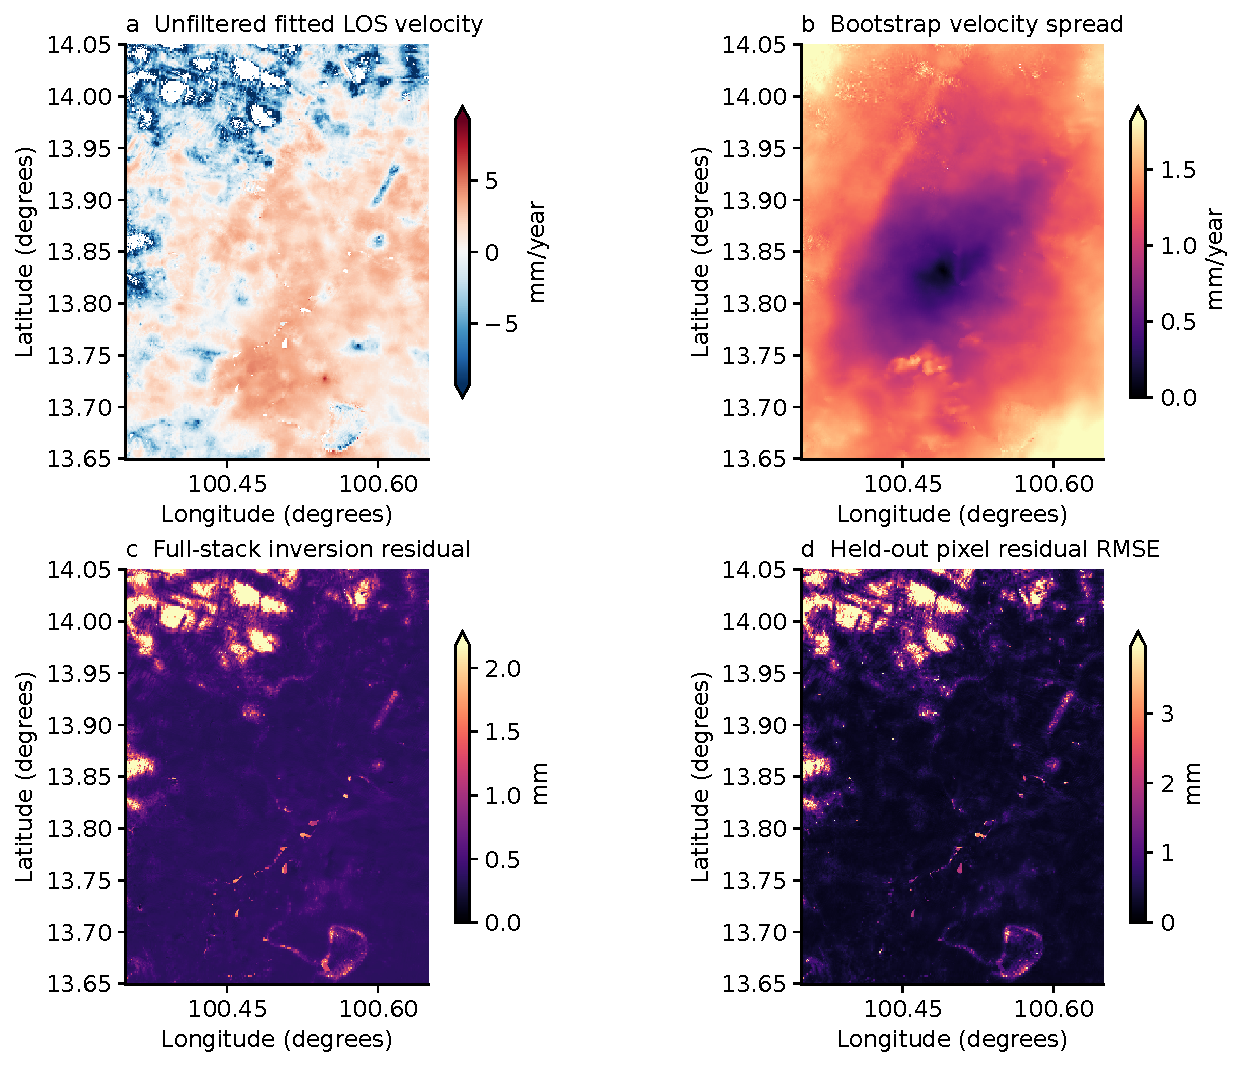
\includegraphics[width=\linewidth]{figures/S3_matched_quality.pdf}
\caption{Actual same-chain quality fields in the Bangkok processing rectangle. Panel a shows the unfiltered fitted LOS velocity only where the full quality mask passes. Other panels retain finite quality diagnostics and held-out RMSE. Symmetric velocity limits and the upper limits of other color scales use their 98th percentiles for readability; values outside those limits are clipped in color only and retained in the data. No map supplies independent GNSS accuracy or motion in unobserved locations.}\end{figure}
